\documentclass[conference,onecolumn]{IEEEtran}
\IEEEoverridecommandlockouts
% The preceding line is only needed to identify funding in the first footnote. If that is unneeded, please comment it out.
\usepackage{cite}
\usepackage{amsmath,amssymb,amsfonts}
\usepackage{algorithmic}
\usepackage{graphicx,subcaption}
\usepackage{hyperref}
\usepackage{textcomp}
\usepackage{xcolor}
\usepackage{listings}
\usepackage{enumitem}

\DeclareMathOperator*{\argmax}{arg\,max}
\DeclareMathOperator*{\argmin}{arg\,min}

\def\BibTeX{{\rm B\kern-.05em{\sc i\kern-.025em b}\kern-.08em
    T\kern-.1667em\lower.7ex\hbox{E}\kern-.125emX}}

\IEEEoverridecommandlockouts

\lstset{
    language=Python,             % Set language to Python
    basicstyle=\ttfamily\small,  % Set font to small and monospaced
    keywordstyle=\color{blue},   % Color keywords
    stringstyle=\color{green},   % Color strings
    commentstyle=\color{gray},   % Color comments
    showstringspaces=false,      % Do not display string spaces
    frame=single,                % Add a frame around the code
    breaklines=true              % Line breaks for long lines
}

\begin{document}

\title{\Large Assignment 1 --- Math Fundamentals for Robotics 16-811, Fall 2024}

\author{
    \IEEEauthorblockN{Mukai Yu}
    \IEEEauthorblockA{\textit{MSR, CMU} \\
        Pittsburgh, PA\\
        \href{mailto:mukaiy@andrew.cmu.edu}{mukaiy@andrew.cmu.edu}}
}

\maketitle

\begin{enumerate}[label=\arabic{enumi}.]
    \item Implement the $PA = LDU$ decomposition algorithm discussed in class.
          Do so yourself (in other words, do not merely use predefined Gaussian elimination code in MatLab or Python).
          Simplifications: (i) You may assume that the matrix A is square and invertible. (ii) Do not worry about column interchanges, just row interchanges.

          Demonstrate (in your pdf) that your implementation works properly, on some examples.

          \textbf{Solution:}
          \begin{lstlisting}
def LDU(A: np.ndarray):
    """PA = LDU decomposition algorithm

    Args:
        A (np.ndarray): input array of shape (m, n) where m >= n and A is of rank n

    Returns:
        P (np.ndarray): permutation matrix
        L (np.ndarray): lower triangular matrix
        D (np.ndarray): diagonal matrix
        U (np.ndarray): upper triangular matrix
    """

    # const A
    A = A.copy().astype(float)
    print("input matrix A:\n", A, end="\n\n")

    # verify the input matrix A is valid for LDU decomposition
    assert len(A.shape) == 2, "Input matrix A must be a 2D array"

    n_row, n_col = A.shape
    print("Input matrix A is a {}x{} matrix\n".format(n_row, n_col))

    assert n_row >= n_col, "Input matrix A must have more rows than columns"
    assert np.linalg.matrix_rank(A) == n_col, "Input matrix A must be of full rank"

    # initialize the permutation matrix P, lower triangular matrix L,
    # diagonal matrix D, and upper triangular matrix U
    P = np.eye(n_row, dtype=float)
    L = np.eye(n_row, dtype=float)
    D = np.eye(n_row, dtype=float)
    U = np.zeros((n_row, n_col), dtype=float)

    # solve for PA = LA'
    print("\nSolve for PA = LA':\n")
    A_prime = A.copy()
    for col in range(n_col):
        if A_prime[col, col] == 0:
            if np.max(A_prime[col:, col]) == 0:
                # Should not happen since A is of full rank
                continue
            # find the row with the largest absolute value in the current column
            max_row = np.argmax(np.abs(A_prime[col:, col])) + col
            print("switching row", col + 1, "with row", max_row + 1)
            # swap the current row with the row of the largest value
            # in the current column
            P[[col, max_row]] = P[[max_row, col]]
            A_prime[[col, max_row]] = A_prime[[max_row, col]]
        for row in range(col + 1, n_row):
            L[row, col] = A_prime[row, col] / A_prime[col, col]
            A_prime[row] -= L[row, col] * A_prime[col]

        print(
            "After eliminating column",
            col + 1,
            ":\nP:\n",
            P,
            "\nL:\n",
            L,
            "\nA':\n",
            A_prime,
            end="\n\n",
        )

    print("After solving PA = LA'\nP:\n", P, "\nL:\n", L, "\nA':\n", A_prime)
    print("PA =\n", P @ A, "\nLA' =\n", L @ A_prime, end="\n\n")

    # Solve for A' = DU
    print("\nSolve for A' = DU:\n")
    for row in range(n_col):
        D[row, row] = A_prime[row, row]
        U[row] = A_prime[row] / D[row, row]
        print(
            "After eliminating row",
            row + 1,
            ":\nD:\n",
            D,
            "\nU:\n",
            U,
            end="\n\n",
        )

    print("After solving A' = DU\nD:\n", D, "\nU:\n", U)
    print("A'=\n", A_prime, "\nDU =\n", D @ U)

    # Check if the decomposition is correct
    assert np.array_equal(P @ A, L @ D @ U), "Decomposition is incorrect"

    # Print the final result
    print("\nFinal result:", "\nP:\n", P, "\nL:\n", L, "\nD:\n", D, "\nU:\n", U)

    return P, L, D, U
            \end{lstlisting}

          \begin{figure}[t]
              \centering
              \begin{minipage}[t]{0.3\textwidth}
                  \centering
                  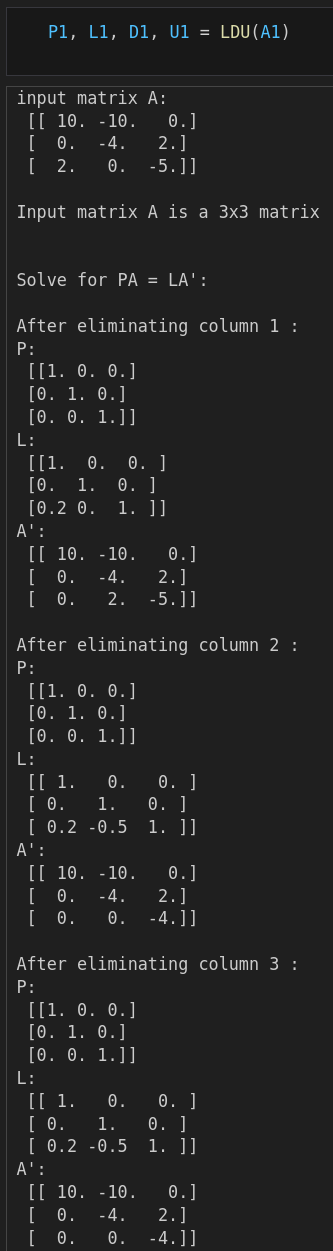
\includegraphics[width=\textwidth]{figs/LDU1.png}
              \end{minipage}%
              \begin{minipage}[t]{0.25\textwidth}
                  \centering
                  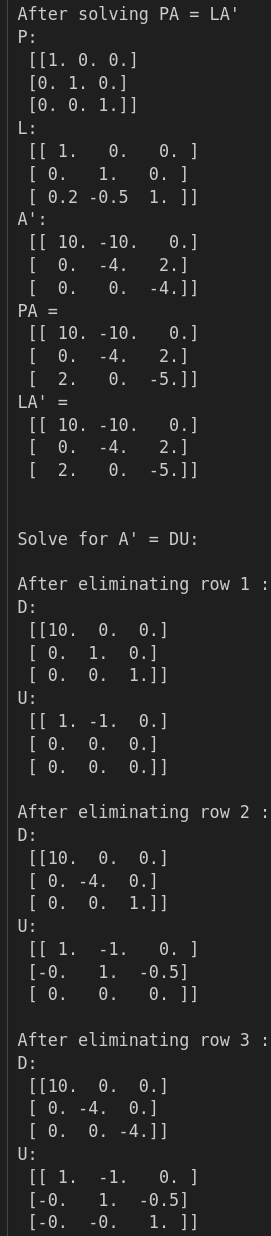
\includegraphics[width=\textwidth]{figs/LDU2.png}
              \end{minipage}%
              \begin{minipage}[t]{0.33\textwidth}
                  \centering
                  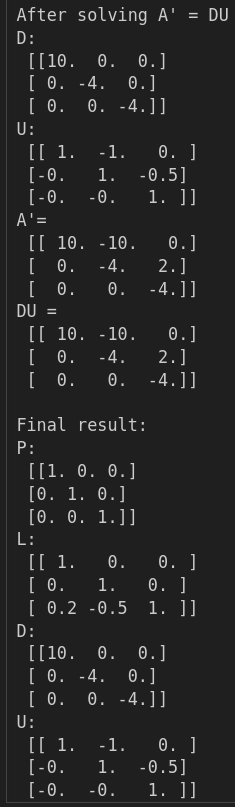
\includegraphics[width=\textwidth]{figs/LDU3.png}
              \end{minipage}
              \caption{Function LDU run on $A_1$ of question 2}
              \label{fig: A_1 LDU}
          \end{figure}

          Refer to my jupyter notebook for the full implementation and demonstration of the LDU decomposition algorithm other than the example given next page.

          \clearpage
    \item Compute the $PA = LDU$ decomposition and the SVD decomposition for each of the following matrices: (In fact, here it is enough to let P be an identity matrix, so A = LDU.)
          \begin{equation*}
              A_1 =
              \begin{pmatrix}
                  10 & -10 & 0  \\
                  0  & -4  & 2  \\
                  2  & 0   & -5
              \end{pmatrix}
              A_2 =
              \begin{pmatrix}
                  5 & -5 & 0  & 0 \\
                  5 & 5  & 5  & 0 \\
                  0 & -1 & 4  & 1 \\
                  0 & 4  & -1 & 2 \\
                  0 & 0  & 2  & 1
              \end{pmatrix}
              A_3 =
              \begin{pmatrix}
                  1  & 1 & 1 \\
                  10 & 2 & 9 \\
                  8  & 0 & 7
              \end{pmatrix}
          \end{equation*}
          You may use any method or tools you wish to solve this problem, including pre-defined
          routines from MatLab or Python, your code, and/or hand calculations.
          (Hand calculations may be easiest for computing the $PA = LDU$ decompositions of these examples. We recommend using pre-defined code to compute the SVD decompositions.)

          Show how you obtained your solutions, that is, show your work, including intermediate steps.

          \textbf{Solution:}

          \textbf{All the intermediate steps of LDU decomposition can be found in the jupyter notebook.}
          Steps of LDU of $A_1$ is shown in Fig.~\ref{fig: A_1 LDU}.

          \begin{enumerate}
              \item \textbf{LDU Decomposition:}
                    \begin{enumerate}
                        \item $A_1$:
                              $$
                                  L_1 =
                                  \begin{pmatrix}
                                      1   & 0    & 0 \\
                                      0   & 1    & 0 \\
                                      0.2 & -0.5 & 1
                                  \end{pmatrix}
                                  D_1 =
                                  \begin{pmatrix}
                                      10 & 0  & 0  \\
                                      0  & -4 & 0  \\
                                      0  & 0  & -4
                                  \end{pmatrix}
                                  U_1 =
                                  \begin{pmatrix}
                                      1 & -1 & 0    \\
                                      0 & 1  & -0.5 \\
                                      0 & 0  & 1
                                  \end{pmatrix}
                              $$
                        \item $A_2$:
                              $$
                                  L_2 =
                                  \begin{pmatrix}
                                      1 & 0    & 0      & 0      & 0 \\
                                      1 & 1    & 0      & 0      & 0 \\
                                      0 & -0.1 & 1      & 0      & 0 \\
                                      0 & 0.4  & -0.667 & 1      & 0 \\
                                      0 & 0    & 0.444  & 0.2083 & 1
                                  \end{pmatrix}
                                  D_2 =
                                  \begin{pmatrix}
                                      5 & 0  & 0   & 0     & 0 \\
                                      0 & 10 & 0   & 0     & 0 \\
                                      0 & 0  & 4.5 & 0     & 0 \\
                                      0 & 0  & 0   & 2.667 & 0 \\
                                      0 & 0  & 0   & 0     & 1
                                  \end{pmatrix}
                                  U_2 =
                                  \begin{pmatrix}
                                      1 & -1 & 0   & 0     \\
                                      0 & 1  & 0.5 & 0     \\
                                      0 & 0  & 1   & 0.222 \\
                                      0 & 0  & 0   & 1     \\
                                      0 & 0  & 0   & 0
                                  \end{pmatrix}
                              $$
                        \item $A_3$: Not applicable since $A_3$ is not full rank.
                    \end{enumerate}
              \item \textbf{SVD Decomposition:}
                    \begin{enumerate}
                        \item $A_1$:
                              \begin{align*}
                                  U_1      & =
                                  \begin{pmatrix}
                                      -0.97502551 & 0.01928246  & -0.22125424 \\
                                      -0.19998937 & -0.50949125 & 0.83691273  \\
                                      -0.09658937 & 0.86025976  & 0.50062326
                                  \end{pmatrix} \\
                                  \Sigma_1 & =
                                  \begin{pmatrix}
                                      14.49778417 & 0          & 0          \\
                                      0           & 5.94733738 & 0          \\
                                      0           & 0          & 1.85564877
                                  \end{pmatrix} \\
                                  V_1^T    & =
                                  \begin{pmatrix}
                                      -0.68585887 & 0.72771207  & 0.00572281  \\
                                      0.3217144   & 0.31024647  & -0.89456524 \\
                                      -0.65276141 & -0.61170439 & -0.44690075
                                  \end{pmatrix}
                              \end{align*}
                        \item $A_2$:
                              \begin{align*}
                                  U_2      & =
                                  \begin{pmatrix}
                                      0.1126266   & 0.86708016  & 0.37480574  & -0.30750061 & -0.0212435  \\
                                      -0.93215705 & 0.15225202  & 0.1626033   & 0.2846251   & 0.0212435   \\
                                      -0.20196646 & 0.2257811   & -0.74973268 & -0.31691184 & -0.4956816  \\
                                      -0.2398716  & -0.41225956 & 0.38334628  & -0.77085017 & -0.17702914 \\
                                      -0.14166742 & 0.06368894  & -0.35217519 & -0.36026217 & 0.84973988
                                  \end{pmatrix} \\
                                  \Sigma_2 & =
                                  \begin{pmatrix}
                                      9.14492811 & 0          & 0          & 0          \\
                                      0          & 7.79814769 & 0          & 0          \\
                                      0          & 0          & 4.42070712 & 0          \\
                                      0          & 0          & 0          & 2.23976139 \\
                                      0          & 0          & 0          & 0
                                  \end{pmatrix} \\
                                  V_2^T    & =
                                  \begin{pmatrix}
                                      -0.44807922 & -0.65407164 & -0.60275097 & -0.09003647 \\
                                      0.65357327  & -0.69875055 & 0.28263403  & -0.06861233 \\
                                      0.60783153  & 0.27645026  & -0.74051747 & -0.07582844 \\
                                      -0.05106685 & 0.08667875  & 0.09188657  & -0.99067443
                                  \end{pmatrix}
                              \end{align*}
                        \item $A_3$:
                              \begin{align*}
                                  U_3      & =
                                  \begin{pmatrix}
                                      -0.08686637 & -0.57077804 & -0.81649658 \\
                                      -0.78592384 & -0.4643889  & 0.40824829  \\
                                      -0.6121911  & 0.67716718  & -0.40824829
                                  \end{pmatrix} \\
                                  \Sigma_3 & =
                                  \begin{pmatrix}
                                      17.2832333 & 0          & 0 \\
                                      0          & 1.51322343 & 0 \\
                                      0          & 0          & 0
                                  \end{pmatrix} \\
                                  V_3^T    & =
                                  \begin{pmatrix}
                                      -0.74312678 & -0.09597244 & -0.66223249 \\
                                      0.1339329   & -0.99096789 & -0.0066797  \\
                                      0.65561007  & 0.09365858  & -0.74926865
                                  \end{pmatrix}
                              \end{align*}
                              Here $\Sigma_3$'s last singular value is smaller than $10^{-15}$, so it's regarded as zero.
                    \end{enumerate}
          \end{enumerate}

          \clearpage
    \item Solve the systems of equations $Ax = b$ for the values of A and b given below.
          For each system, specify whether the system has zero, one, or many exact solutions.
          If a system has zero exact solutions, give “the SVD solution” (as defined in class) and explain what this solution means.
          If a system has a unique exact solution, compute that solution.
          If a system has more than one exact solution, specify both “the SVD solution” and all solutions, using properties of the SVD decomposition of the matrix A, as discussed in class.

          Show your work, including verifying that your answers are correct.

          \begin{enumerate}
              \centering
              \item $A =
                        \begin{pmatrix}
                            10 & -10 & 0  \\
                            0  & -4  & 2  \\
                            2  & 0   & -5
                        \end{pmatrix}
                        b =
                        \begin{pmatrix}
                            10 \\
                            2  \\
                            13
                        \end{pmatrix}
                    $
              \item $A =
                        \begin{pmatrix}
                            1  & 1 & 1 \\
                            10 & 2 & 9 \\
                            8  & 0 & 7
                        \end{pmatrix}
                        b =
                        \begin{pmatrix}
                            1 \\
                            3 \\
                            1
                        \end{pmatrix}
                    $
              \item $A =
                        \begin{pmatrix}
                            1  & 1 & 1 \\
                            10 & 2 & 9 \\
                            8  & 0 & 7
                        \end{pmatrix}
                        b =
                        \begin{pmatrix}
                            3 \\
                            2 \\
                            2
                        \end{pmatrix}
                    $
          \end{enumerate}

          Parts (b) and (c) have the same A matrix but different b vectors.
          You will see that “the SVD solution” is the same for both parts.
          Explain why that makes sense.
          Your explanation should be based on the meaning of the columns of U that arose in A's SVD decomposition.

          \textbf{Solution:}
          \begin{lstlisting}
def solve_systems_of_equations(A: np.ndarray, b: np.ndarray) -> np.ndarray:
    """Solve a system of equations of the form Ax = b for x.

    Args:
        A (np.ndarray): Input matrix A
        b (np.ndarray): Target vector b

    Returns:
        np.ndarray: Solution vector x
    """

    # copy A and b to avoid modifying the original matrices
    A = A.copy()
    b = b.copy()

    # reshape b into a column vector
    b = b.reshape(-1, 1)

    # verify that b has the same number of rows as A
    assert A.shape[0] == b.shape[0], "A and b have different numbers of rows"

    # perform SVD on A
    U, Sigma, Vt = np.linalg.svd(A)

    # factor out extremely small singular values of Sigma
    Sigma = Sigma[Sigma > 1e-10]

    # construct the pseudo-inverse of A
    M_sigma_inverse = np.zeros((U.shape[1], Vt.shape[0]))
    for i in range(len(Sigma)):
        M_sigma_inverse[i][i] = 1 / Sigma[i]
    M_pseudo_inverse = Vt.T @ M_sigma_inverse @ U.T
    print("pseudo inverse of matrix A:\n", M_pseudo_inverse)

    # compute the "solution" to the system of equations
    x = M_pseudo_inverse @ b
    return x
          \end{lstlisting}

          \begin{enumerate}
              \item $A =
                        \begin{pmatrix}
                            10 & -10 & 0  \\
                            0  & -4  & 2  \\
                            2  & 0   & -5
                        \end{pmatrix}$'s a full rank matrix, so its column space spans $\mathbb{R}^3$, and thus its systems of equations all have a unique exact solution.

                    $$
                        A^{\dagger} =
                        \begin{pmatrix}
                            0.125 & -0.3125 & -0.125 \\
                            0.025 & -0.3125 & -0.125 \\
                            0.05  & -0.125  & -0.25
                        \end{pmatrix}
                        x =
                        \begin{pmatrix}
                            -1 \\
                            -2 \\
                            -3
                        \end{pmatrix}
                    $$
              \item $A =
                        \begin{pmatrix}
                            1  & 1 & 1 \\
                            10 & 2 & 9 \\
                            8  & 0 & 7
                        \end{pmatrix}$'s a rank 2 matrix, so its column space spans a 2D subspace of $\mathbb{R}^3$, and thus its systems of equations have many solutions.
                    It's easy to see that the row space of $A$ is spanned by the first two rows of $A$:
                    $$
                        1 \cdot ROW_2 - 2 \cdot ROW_1 = ROW_3
                    $$
                    Columns of $U$ corresponding to the zero singular values span the null space of $A$.

                    The SVD solution is:
                    $$
                        A^{\dagger} =
                        \begin{pmatrix}
                            -0.04678363 & -0.00730994 & 0.08625731  \\
                            0.37426901  & 0.30847953  & -0.44005848 \\
                            0.00584795  & 0.03216374  & 0.02046784
                        \end{pmatrix}
                        \bar{x} =
                        \begin{pmatrix}
                            0.01754386 \\
                            0.85964912 \\
                            0.12280702
                        \end{pmatrix}
                    $$
                    Where $\bar{x}$ is not exact.
              \item Similar to part (b), the SVD solution is the same as part (b) since the matrix $A$ is not full rank.

                    The SVD solution is:
                    $$
                        A^{\dagger} =
                        \begin{pmatrix}
                            -0.04678363 & -0.00730994 & 0.08625731  \\
                            0.37426901  & 0.30847953  & -0.44005848 \\
                            0.00584795  & 0.03216374  & 0.02046784
                        \end{pmatrix}
                        \bar{x} =
                        \begin{pmatrix}
                            0.01754386 \\
                            0.85964912 \\
                            0.12280702
                        \end{pmatrix}
                    $$
                    Where $\bar{x}$ is also not exact.
          \end{enumerate}

          \clearpage
    \item Suppose that $u$ is an n-dimensional column vector of unit length in $\mathbb{R}^n$, and let $u^T$ be its transpose.
          Then $uu^T$ is a matrix.
          Consider the $n \times n$ matrix $A = I - uu^T$.
          \begin{enumerate}
              \item Describe the action of the matrix A geometrically.
              \item Give the eigenvalues of A.
              \item Describe the null space of A.
              \item What is $A^2$?
          \end{enumerate}
          (As always, show your work.)

          \textbf{Solution:}
          \begin{enumerate}
              \item $Ax$ represents the operation of projecting vector $x$ onto the hyperplane orthogonal to $u$.
                    $$
                        Ax = (I - uu^T)x = x - u(u^Tx) = x - (u^Tx)u
                    $$
                    The amount of projection of $x$ onto $u$ is $u^Tx$.
                    Subtracting this projection from $x$ gives the projection of $x$ onto the hyperplane orthogonal to $u$.
              \item The eigenvalues of $A$ are 1 and 0.
                    Definition of eigenvalues:
                    \begin{align*}
                        det(A - \lambda I) & = det(I - uu^T - \lambda I)      \\
                                           & = det((1 - \lambda)I - uu^T) = 0
                    \end{align*}
                    \begin{enumerate}
                        \item For any vector $x$ orthogonal to $u$:
                              $$
                                  Ax = (I - uu^T)x = x - (u^Tx)u = x
                              $$
                        \item For any vector $x$ parallel to $u$:
                              $$
                                  Ax = (I - uu^T)x = x - (u^Tx)u = x - x = 0
                              $$
                    \end{enumerate}
              \item The null space of $A$ is the subspace spanned by $u$, because any vector $x$ parallel to $u$ will be projected to $\overrightarrow{0}$.
                    $$
                        Au = (I - uu^T)u = u - uu^Tu = u - u = 0
                    $$
              \item $A^2 = (I - uu^T)^2 = I - 2uu^T + uu^Tuu^T = I - uu^T = A$.
          \end{enumerate}

          \clearpage
    \item The following problem arises in a large number of robotics and vision problems: Suppose $p_1, . . . , p_n$ are the 3D coordinates of n points located on a rigid body in three-space.
          Suppose further that $q_1, . . . , q_n$ are the 3D coordinates of these same points after the body has been translated and rotated by some unknown amount.
          Derive an algorithm in which SVD plays a central role for inferring the body's translation and rotation.
          (You may assume that the coordinate values are precise not noisy, but see comment and caution below.)

          Show (in your pdf) that your algorithm works correctly by running it on some examples.

          \textbf{Comment:} This problem requires some thought.
          There are different approaches.
          Although you can find a solution on the web or in a vision text book, try to solve the problem yourself before looking at any such sources.
          Spend some time on the problem.
          It is good practice to develop your analytic skills.
          Feel free to discuss among yourselves.
          (As always, cite any sources, including discussions with others.)

          \textbf{Requirement:} Your algorithm should make use of all the information available.
          True, in principle you only need three pairs of points -- but if you use more points your solution will be more robust, something that might come in handy some day when you need to do this for real with noisy data.

          \textbf{Caution:} A common mistake is to derive an algorithm that finds the best affine transformation, rather than the best rigid body transformation.
          Even though you may assume precise coordinate values, imagine how your algorithm would behave with noise.
          Your algorithm should still produce a rigid body transformation.

          \textbf{Hint:} Suppose for a moment that both sets of points have the origin as centroid.
          Assemble all the points {$p_i$} into a matrix P and all the points {$q_i$} into another matrix Q.
          Now think about the relationship between P and Q.
          You may wish to find a rigid body transformation that minimizes the sum of squared distances between the points {$q_i$} and the result of applying the rigid body transformation to the points {$p_i$}.

          You may find the following facts useful (assuming the dimensions are sensible):
          $$
              \|x\|^2 = x^Tx,
              x^TR^Ty = Tr(Rxy^T).
          $$
          [Here x and y are column vectors (e.g., 3D vectors) and R is a matrix (e.g., a 3 x 3 rotation matrix).
                  The superscript T means transpose, so $x^Tx$ is a number and $xy^T$ is a matrix.
                  Also, Tr is the trace operator that adds up the diagonal elements of its square matrix argument.]

          You will have more complicated expressions for x and y, involving the points {$p_i$} and {$q_i$}.

          \textbf{Solution:}
          The realistic version of the problem's solution is the point-to-point \href{https://en.wikipedia.org/wiki/Iterative_closest_point}{\textit{iterative closest point (ICP) algorithm}} for point cloud matching/alignment, where the index of the points in the 2 point clouds are not matched, and even if they match, the points are not perfectly aligned due to imperfect perception.
          In more challenging scenario, we could even have missing chunks of points in one of the point clouds, where we need to use point-to-plane ICP algorithm.

          Regardlessly, the objective is to find:
          $$
              \argmin_{T \in SE(3)} \sum_{i = 1}^n \|\dot{q_i} - T\dot{p_i}\|^2
          $$
          Where $\dot{q_i}$ and $\dot{p_i}$ are the homogeneous coordinates of $q_i$ and $p_i$ respectively.

          This is equivalent to find:
          $$
              \argmin_{R \in SO(3), t \in \mathbb{R}^3} \sum_{i = 1}^n \|q_i - (Rp_i + t)\|^2
          $$
\end{enumerate}

\end{document}
